\section{Numerical Validation Protocol}
\label{sec:numerical_protocol}

\paragraph{Validation target.}
This section specifies a minimal validation suite aligned with the theory sections on involution,
orientation gauge, and composed representative action. The goal is not broad
benchmarking, but targeted falsification of the duality identities.

\subsection{Single core figure specification}

\begin{figure*}[t]
  \centering
  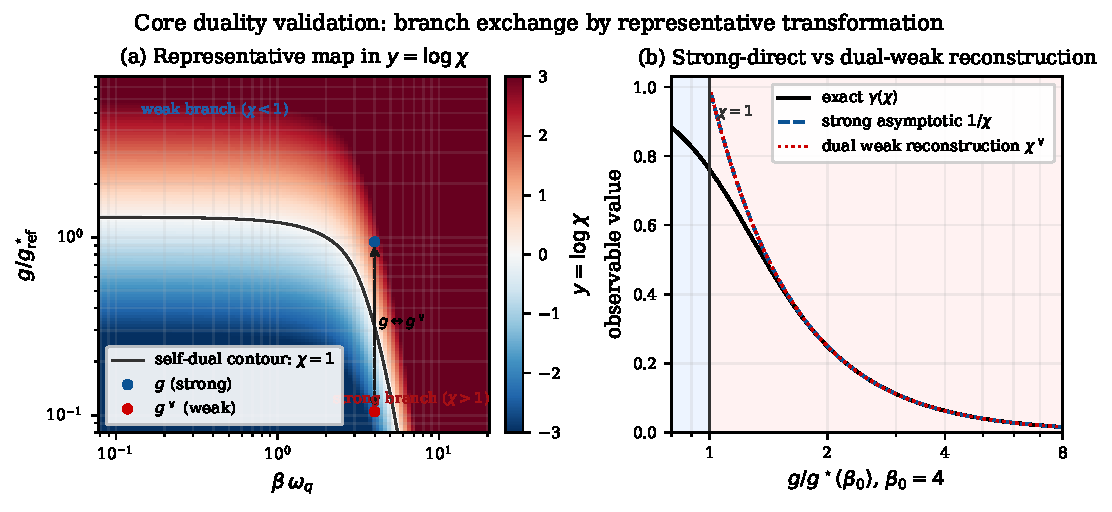
\includegraphics[width=0.86\textwidth]{../figures/hmf_dual_map_core.pdf}
  \caption{
  Core dual-representative validation.
  \textbf{(a)} Diverging \(y=\log\chi\) map in \((\beta,g)\), with the self-dual contour
  \(\chi=1\), explicit weak/strong branch labels, and a fixed-\(\beta\) representative pair
  \(g\leftrightarrow g^\vee\).
  \textbf{(b)} Line-style decoding of asymptotic exchange at fixed \(\beta_0\):
  black solid \(=\gamma(\chi)\) exact, blue dashed \(=1/\chi\) (strong asymptotic),
  red dotted \(=\chi^\vee=\chi(\beta_0,g^\vee,\theta)\) (dual weak variable).
  Convergence on the strong side (\(g/g^\star>1\)) visualizes the control-regime transfer claim.
  }
  \label{fig:core_dual_map}
\end{figure*}

\paragraph{Implementation note.}
The figure is produced by \path{paper_dual_hmf/validation/make_core_dual_map_figure.py}, which
is self-contained by design and writes outputs to
\path{paper_dual_hmf/manuscript/figures/}.

\subsection{Exact versus analytic agreement degree}

\begin{figure}[tbp]
  \centering
  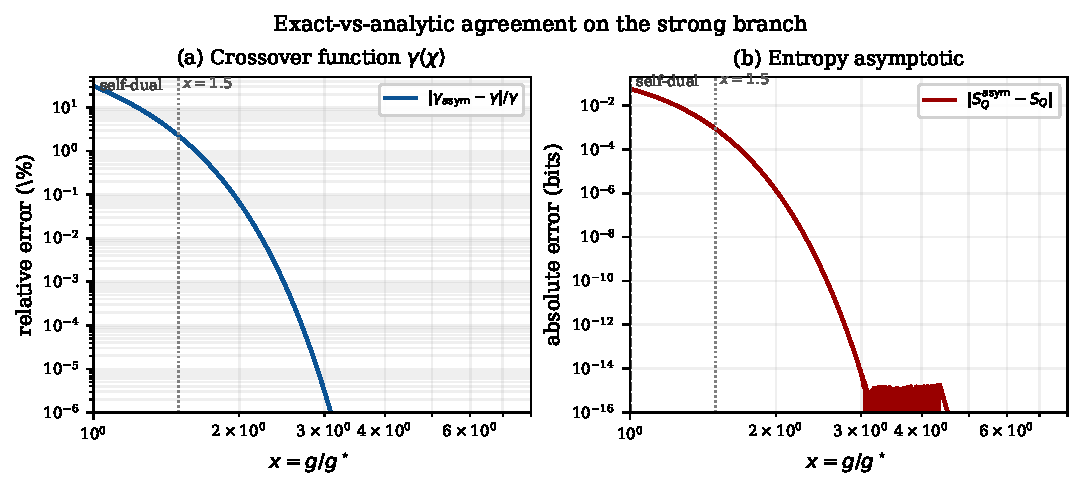
\includegraphics[width=\columnwidth]{../figures/hmf_exact_vs_analytic_error.pdf}
  \caption{
  Quantitative agreement diagnostics between exact closure expressions and analytic asymptotics on
  the strong branch \(x:=g/g^\star\ge 1\).
  \textbf{(a)} Relative error of \(\gamma_{\mathrm{asym}}=1/\chi\) against
  \(\gamma_{\mathrm{exact}}=\tanh\chi/\chi\) with \(\chi=x^2\).
  \textbf{(b)} Absolute entropy error in bits for
  \(S_Q^{\mathrm{asym}}=((1+2\chi)e^{-2\chi})/\ln 2\) against exact
  \(S_Q=h_2\!\left((1+|\tanh\chi|)/2\right)\).
  The dominant mismatch is localized near the crossover; errors collapse rapidly for \(x\gtrsim1.5\).
  }
  \label{fig:exact_vs_analytic_error}
\end{figure}

\begin{table}[tbp]
  \caption{Agreement degree in fixed strong-branch windows \(x\ge x_{\min}\), with
  \(\delta_\gamma:=|\gamma_{\mathrm{asym}}-\gamma_{\mathrm{exact}}|/\gamma_{\mathrm{exact}}\) and
  \(\Delta S_Q:=S_Q^{\mathrm{asym}}-S_Q^{\mathrm{exact}}\). Entries for \(\delta_\gamma\) are in
  percent, and entries for \(|\Delta S_Q|\) are in bits.}
  \label{tab:exact_vs_analytic_metrics}
  \begin{ruledtabular}
  \begin{tabular}{ccccc}
    \(x_{\min}\) & \(\max \delta_\gamma\) & \(\mathrm{RMS}\,\delta_\gamma\) & \(\max | \Delta S_Q |\) & \(\mathrm{RMS}\,| \Delta S_Q |\) \\
    \hline
    1.0 & 31.30\% & 6.68\% & \(5.87\times10^{-2}\) & \(1.08\times10^{-2}\) \\
    1.2 & 11.87\% & 2.33\% & \(1.45\times10^{-2}\) & \(2.30\times10^{-3}\) \\
    1.5 & 2.24\% & 0.389\% & \(8.79\times10^{-4}\) & \(1.16\times10^{-4}\) \\
    2.0 & 0.0668\% & 0.00978\% & \(1.37\times10^{-6}\) & \(1.48\times10^{-7}\) \\
  \end{tabular}
  \end{ruledtabular}
\end{table}

\paragraph{Interpretation.}
Yes, the exact and analytic forms agree to high precision once the analysis is in the intended
strong-asymptotic region.
At the self-dual neighborhood (\(x\approx1\)), disagreement is expected because asymptotics are
not yet controlled.
By \(x\ge1.5\), \(\gamma\)-errors are already at the few-percent level (max \(2.24\%\)), while
entropy errors are below \(10^{-3}\) bits.
By \(x\ge2\), agreement is effectively exact for manuscript purposes:
\(<10^{-3}\) relative error for \(\gamma\) and \(O(10^{-6})\) bits for entropy.

\paragraph{Implementation note.}
Figure~\ref{fig:exact_vs_analytic_error} and
Table~\ref{tab:exact_vs_analytic_metrics} are generated from
\path{paper_dual_hmf/validation/make_exact_vs_analytic_comparison.py}
with numeric output written to
\path{paper_dual_hmf/validation/output/exact_vs_analytic_metrics.csv}.

\subsection{Acceptance checks}

\begin{enumerate}
  \item Algebraic: \((g^\vee)^\vee=g\) and \(\chi(\beta,g^\vee,\theta)=1/\chi(\beta,g,\theta)\).
  \item Orientation: \(\beff'+\beff=2\beta\), and radial invariants are orientation-even.
  \item Asymptotic exchange: strong-branch direct evaluation agrees with dual weak-branch expansion in target limits.
  \item Manuscript: compile pass with theorem/interpretation tagging complete.
\end{enumerate}

\subsection{Data and script reuse policy}
Reuse existing crossover and involution plotting pipelines first; avoid heavy new ED campaigns in
this phase.
